\documentclass[a4paper, 12pt]{book}
\usepackage[a4paper, left=0.5in, right=0.5in, top=0.8in, bottom=0.8in]{geometry}

\usepackage{hyperref} % this generates the bookmarks for PDFs
\usepackage[english]{babel}
\usepackage{amsfonts} % for math sets letters
\usepackage{amsmath} % for general math stuff
\usepackage{amssymb} % for general math stuff
\usepackage{blindtext} % generates filler text
\usepackage{paralist} % for the compactenum and compactlist procedures
\usepackage{pgfplots} % for tikz
\usepackage{tikz} % for tikz

\usetikzlibrary{quotes}
\usetikzlibrary{shapes}
\usetikzlibrary{matrix}
\usetikzlibrary{positioning}
\usetikzlibrary{arrows.meta}

\setlength{\unitlength}{1cm}

% ====== MY MACROS

\newcommand{\TUG}{\TeX\ Users Group}
\newcommand{\kw}[2][\bfseries]{{#1#2}}
\newcommand{\im}[1]{{\(#1\)}}
\newcommand{\cm}[1]{{\[#1\]}} % remember that when you want to do center math you don't need to have \\ on EOL
\newcommand{\head}[1]{\textnormal{\textbf{#1}}}
\newtheorem{thm}{Theorem}
\newtheorem{dfn}[thm]{Definition}

% ====== MY MACROS

\title{TikZ introduction}
\author{Me}
\date{Jan 28, 2024}

\addtocontents{toc}{\protect{\pdfbookmark[0]{\contentsname}{toc}}}

\begin{document}
\maketitle
\tableofcontents
\chapter{TikZ Basics}
\section{\LaTeX\ built-in drawing functions}
\LaTeX\ has some basic drawing capabilities built-in, as:\\\\
\begin{picture}(1,1)
\put(0,0) {\circle{1}}    
\put(-0.5, 0) {\line(1,0){1}}
\put(-0.3, 0.06){text}
\end{picture}\\\\
This is not that good and there are a lot of other packages that works in a similar faction. TikZ is diffrent, because it allows you to \textit{program} graphics with code, witch provides more consistence and a more pleasant look. Here's how to do it in the TikZ way:\\\\
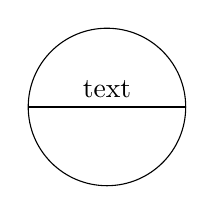
\begin{tikzpicture}
    \draw circle (1.0);
    \draw (-1,0) to ["text"] (1,0);
\end{tikzpicture}
\newpage
\section{Creating the first TikZ images}
Lets now start to draw a \textbf{grid}.\\\\
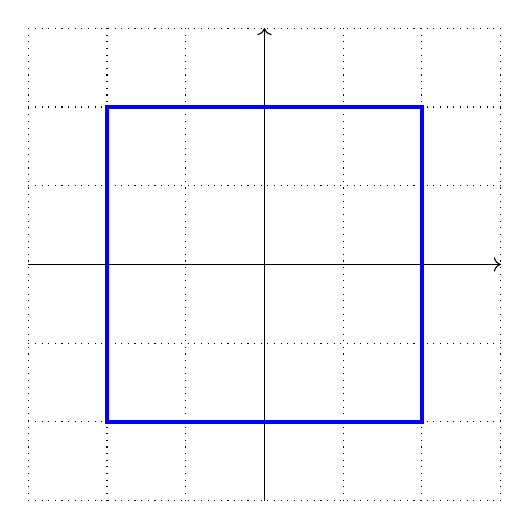
\begin{tikzpicture}
    \draw[thin,dotted] (-3, -3) grid (3, 3); % from coordinate (-3,-3) to (3,3), [thin,dotted] is the option for the line
    \draw[->] (-3, 0) -- (3, 0); % draws the horizontal axis
    \draw[->] (0, -3) -- (0, 3); % draws the vertical axis
    \draw[very thick, blue] (-2, -2) -- (-2, 2) -- (2, 2) -- (2, -2) -- cycle;
    %\draw[very thick, blue] (-2, -2) -- (-2, 2) -- (2, 2) -- (2, -2) -- (-2, -2); % it does the same thing
\end{tikzpicture}\\\\
Now let's try Polar Coordinates. Before we were using cartesian coordinates. But now we will deal with angle and distance-based coordinates.\\\\
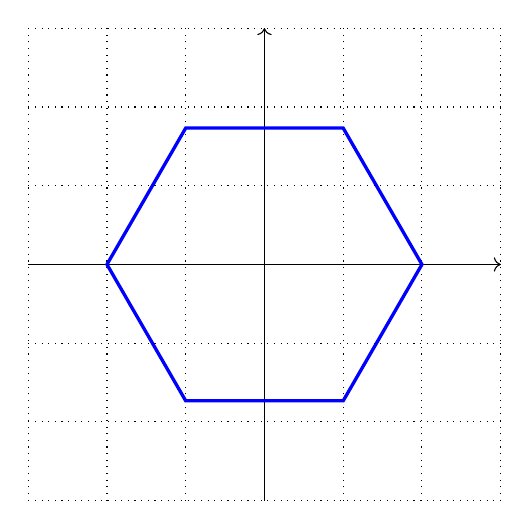
\begin{tikzpicture}
    \draw[thin,dotted] (-3, -3) grid (3, 3);
    \draw[->] (-3, 0) -- (3, 0);
    \draw[->] (0, -3) -- (0, 3);
    \draw[very thick, blue] (0:2) -- (60:2) -- (120:2) -- (180:2) -- (240:2) -- (300:2) -- cycle; % this syntax is (angle:distance_to_origin)
\end{tikzpicture}\\\\
If we are using cartesian coordinates, we can also use relative coordinates with the syntax \texttt{++(1,0)}.
\subsection{Drawing other shapes with TikZ}
We can do a lot of stuff with it.\\\\

\begin{tikzpicture}
    \draw (-3, -3) rectangle (3, 3);
    \draw[blue, fill=yellow] (0,0) circle [radius=2];
    \draw[shading=ball, ball color=white] (-0.5, 0.5,0) ellipse [x radius=0.2, y radius=0.4];
    \draw[blue, fill=black] (0.5, 0.5,0) ellipse [x radius=0.2, y radius=0.4];
    \draw (-1, -1) arc [start angle=185, end angle=355, x radius=1, y radius=0.5];
\end{tikzpicture}
\newpage
\section{Nodes}
Yeap, we can draw nodes.\\\\
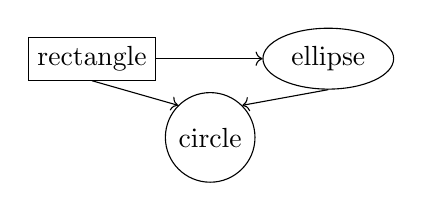
\begin{tikzpicture}
    \node (r) at (0,1) [draw, rectangle] {rectangle};
    \node (c) at (1.5,0) [draw, circle] {circle};
    \node (e) at (3,1) [draw, ellipse] {ellipse};
    \draw[->] (r.east) -- (e.west);
    \draw[->] (r.south) -- (c.north west);
    \draw[->] (e.south) -- (c.north east); % note that r. c. and e. are used to reference the nodes
\end{tikzpicture}\\\\
In TikZ these compass directions are called \textbf{anchors}, that's because we can use them to anchor a node on a position.\\\\
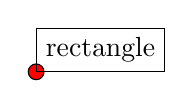
\begin{tikzpicture}
    \draw[fill=red] (4, 2) circle [radius=0.1];
    \node at (4,2) [draw, rectangle, anchor=south west] {rectangle}; % the 'at (4, 2) is what ties these two structures togheder
\end{tikzpicture}\\\\
While rectangle and circle nodes are available by default, others requires the \texttt{shapes} package. All these shapes, like the \texttt{rectangle} and \texttt{circle} ones provides anchors that on can refeer to if you want to tie it togheder with other stucture like a line or other shapes.\\\\
\begin{tikzpicture}
    \coordinate (begin) at (2,0);
    \coordinate (end) at (4,2);
    \draw (begin) -- (end);
\end{tikzpicture}\\\\ % (begin) and (end) are examples of naming that you can use to anchor stuff
% we can also define outer sep and inner sep (and xsep/ysep) to setup separations between nodes
\newpage
\section{Drawing Edges and Arrows}

\begin{tikzpicture}
    \node (tex) [fill=orange, text=white] {TEX};
    \node (pdf) [fill={rgb:red,244;green,15;blue,2}, text=white, right=of tex] {PDF};
    \draw (tex) edge[->] node[font=\tiny\ttfamily, above] {pdflatex} (pdf);
\end{tikzpicture}\\\\ 
We can also use custom arrow types, like:\\\\
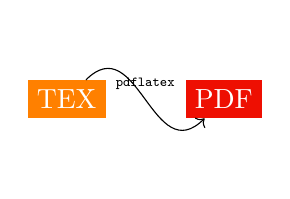
\begin{tikzpicture}
    \node (tex) [fill=orange, text=white] {TEX};
    \node (pdf) [fill={rgb:red,244;green,15;blue,2}, text=white, right=of tex] {PDF};
    \draw[->] (tex) to[out=45, in=225, looseness=1.5] node[font=\tiny\ttfamily, above] {pdflatex} (pdf);
\end{tikzpicture}\\\\ 

\begin{tikzpicture}
    \node (tex) [fill=orange, text=white] {TEX};
    \node (pdf) [fill={rgb:red,244;green,15;blue,2}, text=white, right=of tex] {PDF};
    \draw (tex) edge[very thick, -{Rectangle}] node[font=\tiny\ttfamily, above] {pdflatex} (pdf);
\end{tikzpicture}\\\\ 
\newpage
\section{Using styles and pictures}
We will now understand how to use styles. They are basically a tool the user can define to be used on the various TikZ objects.\\\\

\begin{tikzpicture}
    % \node (A) {A}; % this is the simple example, without styling
    \node [font = \sffamily\bfseries, text = white, shape = circle, ball color = blue] (A) {A}; % this is styling
    \draw (A);
\end{tikzpicture}\\\\
Being honest two, the simple, unstyled graphs are much better and all I need anyways.\\\\
But yeah, you can define styles locally and globally we you really need it.
\newpage
\section{Drawing Trees and Graphs}
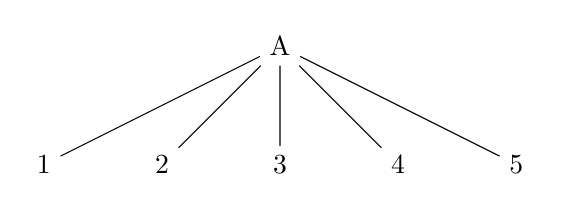
\begin{tikzpicture}
    \node (a) {A} 
    child { node {1} edge from parent}
    child { node {2} edge from parent}
    child { node {3} edge from parent}
    child { node {4} edge from parent}
    child { node {5} edge from parent}
    ;
    \draw (a);
\end{tikzpicture}\\\\
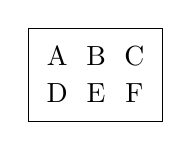
\begin{tikzpicture}
    \node [matrix, draw]
    {
        \node {A};  & \node{B}; & \node{C}; \\
        \node {D};  & \node{E}; & \node{F}; \\
    };
\end{tikzpicture}\\\\
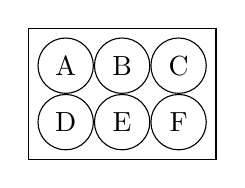
\begin{tikzpicture}
    \matrix [matrix of nodes, draw, nodes = {circle, draw, minimum width=2em}] 
    {
        A & B & C \\
        D & E & F \\
    };
\end{tikzpicture}\\\\
From now on we are just skipping large portions of the textbook because they are boring and I don't see any need for them right now. Maybe we will be back for it.
\newpage
\section{Drawing smooth curves}
Now we enter in a section what will be useful for when we actually deal with math.\\\\
\begin{tikzpicture}
    \begin{axis}[axis lines=center]
        \addplot[domain=-3:3, smooth, thick] { x^3 - 5*x };
    \end{axis}
\end{tikzpicture}\\\\
As you can see. This is not that hard!\\\\
For a really long time, this object along with matrices, nodes, trees will be enough! Along with what else from algebra and logic may come up.\\\\
Of course, real knowledge will only arise when you are actually writing math and need to solve the problems these constructs will trigger.
\end{document}